\chapter{Ontologien}
\section{Definition}
Ontologien definieren eine Reihe von repräsentativen Primitiven, mit denen ein Wissens- oder Diskursbereich modelliert werden kann. Sie bestehen aus Begriffen und Beziehungen, die einen definierten, abgeschlossenen Problembereich darstellen. \cite{TomGruber.2009}\newline
Ontologien können Kenntnisse und Wissen in einem Bereich auf eine strukturierte und nutzbare Art verfügbar machen. Die vielen Verknüpfungen innerhalb einer Ontologie verleihen ihr eine hohe semantische Ausdrucksstärke. Von vorhandenem Wissen können Rückschlüsse gezogen und weitere Beziehungen und Ableitungsregeln ermittelt werden. \cite{WolfgangHesse.2005}\newline
Ontologien lassen sich mit dreiteiligen Tupeln aufbauen, die nach dem Prinzip „Subjekt-Prädikat-Objekt“ formuliert werden. Hierbei entspricht das Subjekt einem Knoten, das Prädikat einer Kante und das Objekt entweder einem Literalwert oder einem weiteren Knoten. So wäre zum Beispiel \glqq[Eine] Stadt hat Einwohner\grqq{} ein Satz, der einer Ontologie im Bereich der Geografie entnommen werden kann, Wobei \glqq Stadt\grqq{} und \glqq Einwohner\grqq{} jeweils ein Knoten sind und „hat“ die Kante zwischen den Knoten darstellt. \cite{Wikipedia.31.10.201911:12}\newline

Eine einfache Ontologie im Geographischen Bereich könnte zum Beispiel so aussehen:\\

\begin{center}
    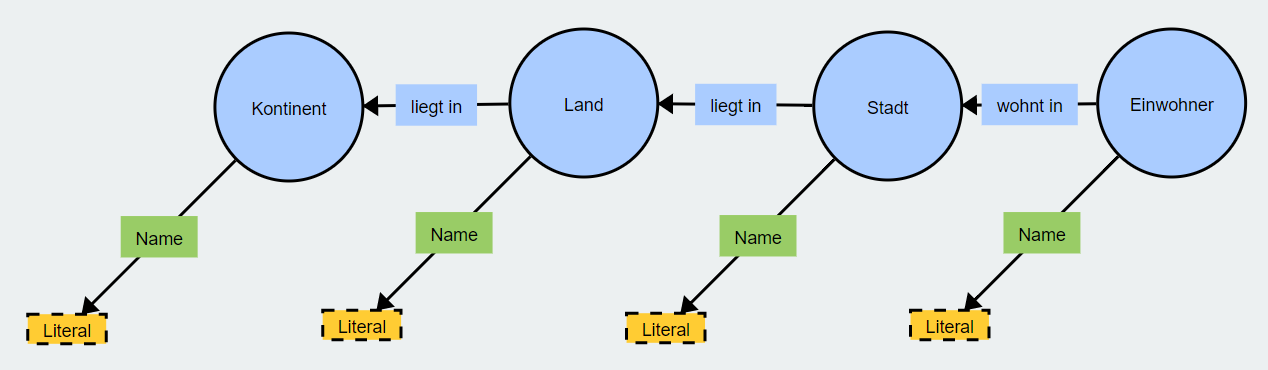
\includegraphics[width=1\textwidth]{Thesis/Images/SampleOntologyLiterals.png}
\end{center}

Um eine Ontologie einzusetzen, beispielsweise bei einer semantischen Suche, werden die Literalwerte verwendet. Diese können dann Wörte bei einer Suche mit den Klassen verbinden. In diesem Beispiel wäre also eine Möglichkeit der Literalwert \glqq Max Mustermann\grqq{}, der der Klasse \glqq Einwohner\grqq{} angehört. Über die Beziehungen kann dann so ermittelt werden, dass \glqq Max Mustermann\grqq{} auf einem Kontinent wohnt, dem beispielsweise der Literalwert \glqq Europa\grqq{} zugehört.
\section{Einsatzbereiche}
Aus den Eigenschaften von Ontologien ergeben sich mehrere Einsatzmöglichkeiten. Zum Einen werden Ontologien verwendet, um Wissen zu strukturieren und einen Datenaustausch zu ermöglichen. Außerdem sind sie nicht auf niedrige Datentypen angewiesen und ermöglichen so das Zusammenführen von umfangreichen heterogenen Daten. Sie erleichtern das Suchen innerhalb von Wissensbeständen und damit auch das Editieren einzelner Informationen. Ebenso können Begriffe miteinander verknüpft werden \cite{BernersLee.2001}, wodurch beispielsweise Synonyme oder Homonyme bei einer Suche berücksichtigt werden können.\newline
Einsatzbereiche von Ontologien sind zum Beispiel die Meeresbiologie. Forschungsergebnisse über Flora und Fauna werden gesammelt und unterstützen so die Forschung über Spezies und Biodiversität \cite{Garoufallou.2013}.
Ebenso werden im medizinischen Bereich Ontologien eingesetzt um Symptome, Medikamente und Patientendaten zu verknüpfen und dadurch Diagnosen zu ermitteln und Behandlungsmöglichkeiten zu suchen \cite{WolfgangHesse.2005}.\newline
Ebenso sind Ontologien für das \glqq Semantic Web\grqq{} von hoher Bedeutung, da sie das Verknüpfen verschiedener Seiten und Begriffe unterstützen \cite{BernersLee.2001} und durch das Verwalten von Metadaten das Anwenden einer semantischen Suche ermöglichen. \newline
In allen Bereichen, in denen Entscheidungen anhand von Erfahrung und Wissen getroffen werden oder Informationen strukturiert werden müssen, um sie effektiv nutzen zu können, rentiert sich der Einsatz von Ontologien.\newline
Das trifft auch auf den Bereich des Produkttestens zu. Das Wissen, dass hier verwaltet werden muss, ist die Vielzahl der Testfälle die sich für ein Produkt ermitteln lassen sowie der Zusammenhang zwischen den getesteten Funktionen mit den Modulen, aus denen ein System besteht. Eine Ontologie ist in der Lage, diese unterschiedlichen Informationen in einer Einheit unterzubringen und so das Arbeiten der Verantwortlichen für Produktqualität zu unterstützen.
\section{Erstellung}
Um zu verstehen, wie Produkttesten in eine Ontologie integriert werden kann, wird anhand des Beispiels des BAYOOSOFT Access Managers eine Ontologie schrittweise aufgebaut. Die Testfälle wurde bereits im Rahmen des Praxisprojekts ermittelt und werden jetzt als Grundlage für die Ontologie verwendet. Die Ontologie wurde in Protégé entworfen und mit webVOWL visualisiert. \newline
In folgendem Beispiel werden Funktion und Testfälle des Verwaltens von Berechtigungen zunächst stark einfacht modelliert:\\

\begin{center}
    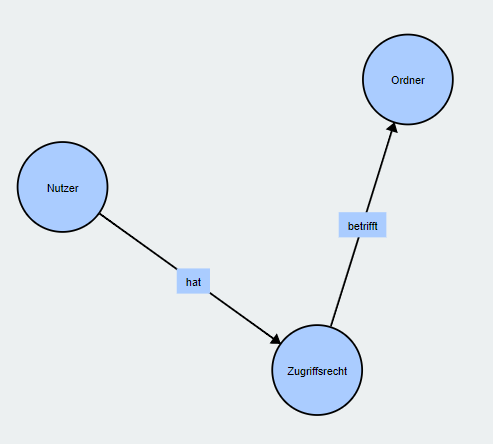
\includegraphics[width=1\textwidth]{Thesis/Images/OntologySmall.png}        
\end{center}

Die Ontologie fasst die Funktion des Berechtigungsmanagements in 3 Klassen mit 2 Beziehungen zusammen. Sie stellt das Zusammenspiel von Usern, Zugriffsrechten und Ordnern dar, aber umfasst offensichtlicherweise nicht alle Aspekte des Produkts und seiner Berechtigungsverwaltung. Im nächsten Schritt wird die Ontologie erweitert, um Sonderfälle und technische Einschränkungen zu berücksichtigen.\\

\begin{center}
    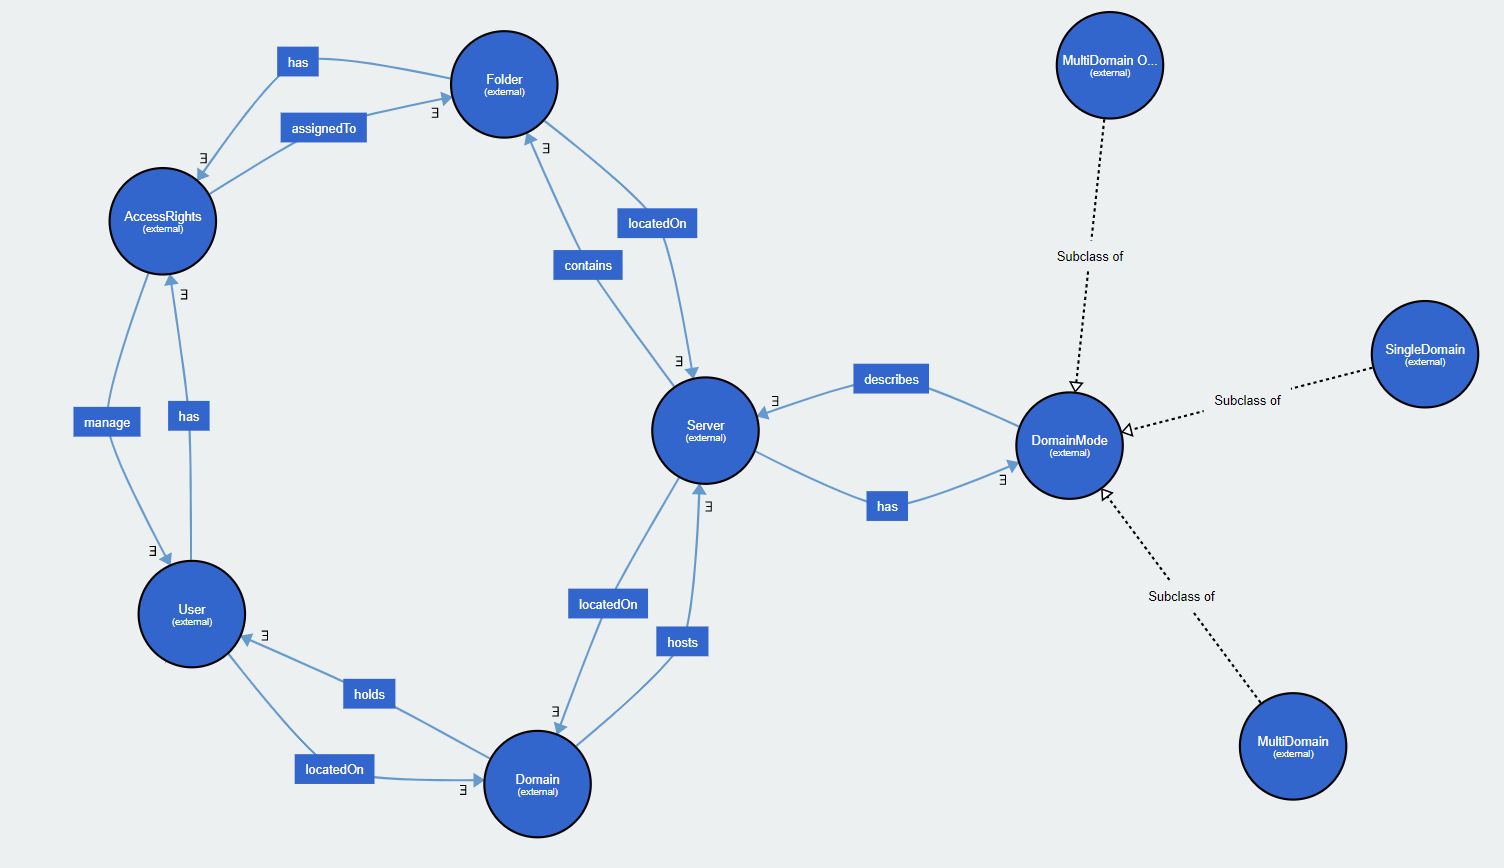
\includegraphics[width=1\textwidth]{Thesis/Images/OntologyBig.png}
\end{center}

Durch diese Erweiterungen werden in der Ontologie noch Domänen einbezogen, auf denen sich User und Server, beziehungsweise impliziert auch Ordner befinden, sowie zusätzlich Domainmodes, die jeweils entsprechend der Domäne regeln können, ob ein Nutzer berechtigt werden kann oder nicht. Dadurch wird sowohl das System realitätsnaher dargestellt, als auch mehr Testfälle einbezogen. Um die Ontologie jedoch verwenden zu können werden noch weitere Schritte benötigt. Zum einen sollte die Ontologie um Funktionsbereiche erweitert werden, da sie in dieser spezifischen Form wenig Nutzen in Bezug auf die im nächsten Kapitel behandelte semantische Suche bringt. \\

\begin{center}
    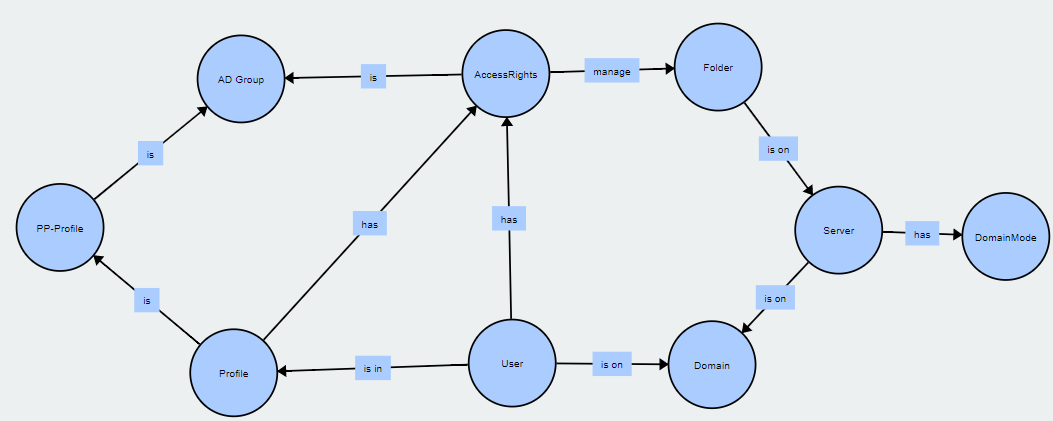
\includegraphics[width=1\textwidth]{Thesis/Images/OntologyProfile.png}
\end{center}

Dazu werden einmal noch Profile und ihre entsprechenden Einschränkungen und Spezialisierungen angefügt. Profile sind ein Teil der Berechtigungsverwaltung und beeinflussen dazu auch die Art, in der im Active Directory gearbeitet wird beziehungsweise, wie ein Nutzer Zugriff auf einem Ordner erlangen kann. Dadurch können mehr und auch breit gefächerte Testfälle in der Ontologie modelliert werden. Im letzten Schritt geht es noch daran, die Ontologie so zu gestalten, das schließlich auch Literalwerte, die für die semantische Suche benötigt werden, mit den entsprechenden Klassen verknüpft werden können. 

\begin{center}
    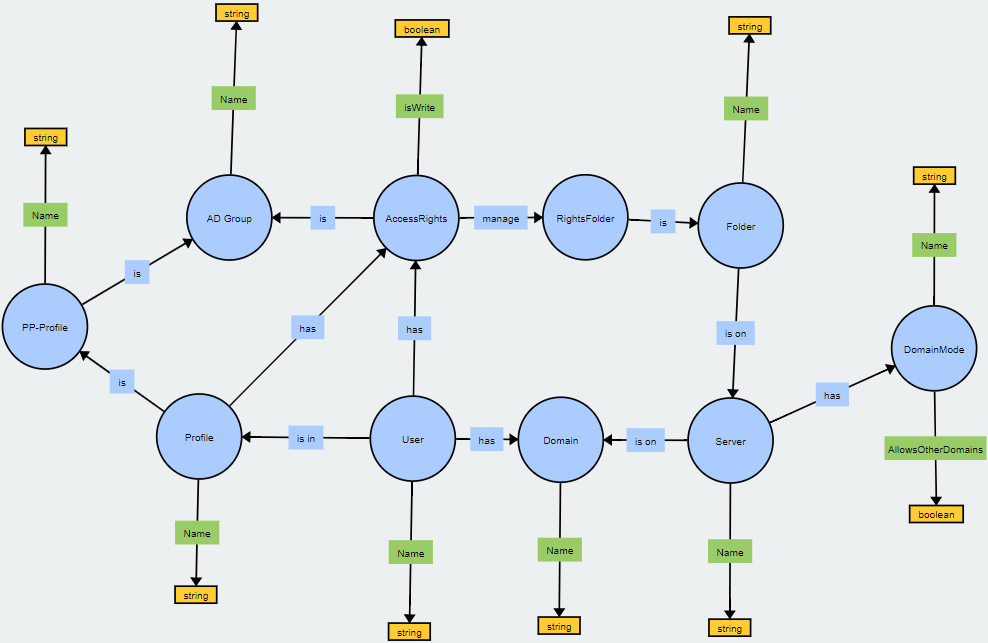
\includegraphics[width=1\textwidth]{Thesis/Images/OntologyLiterals.png}
\end{center}

Um die Ontologie übersichtlicher zu halten, wurden hier einfache Literale wie \glqq Name \grqq{} oder \glqq IsWrite\grqq{} gewählt, welche die Realität nicht vollständig wiederspiegeln, aber für den Rahmen dieser Hausarbeit genügen sollten. Durch die Literale können zum Beispiel die Regeln der Domainmodes bezüglich Fremddomänennutzer mit den Servern verknüpft werden. 